\section{Pretok tekočine}

\subsection{Kvadratna cev}

Prvo sem preizkusil delovanje iterativnih solverjev na preprostem primeru kvadratne cevi, kjer sem uporabil metode Jacobijeve, Gauss-Seidelove iteracije in SOR. Kot robne pogoje sem uporabil vrednost nič na steni in enotski tlači gradient, notranjost pa sem diskretiziral z $N$ točkami po metodi končnih razlik (MKR).

Za SOR potrebujemo faktor nad-relaksacije $\omega$, za kar sem uporabil približek
\begin{equation}\label{eq:omega}
    \omega = \frac{2}{1+ \frac{\pi}{N}},
\end{equation}
kjer je $N$ število točk po koordinatni osi. Uporabil sem tudi Čebišev pospešek, kjer sem iteracije izvajal izmenično po belih in črnih poljih šahovnice in popravljal faktor $\omega$
\begin{align}
    &\omega_0^w = 1 &\omega_0^b = \frac{1}{1-\frac{\rho_{Jac}^2}{2}} \\
    &\omega_n^w = \frac{1}{1 - \frac{\rho_{Jac}^2}{4} \, \omega^w_{n-1}} &\omega_n^b = \frac{1}{1 - \frac{\rho_{Jac}^2}{4} \, \omega^b_{n-1}},\nonumber
\end{align}
ki konvergira k vrednosti v enačbi \ref{eq:omega}. $\rho_{Jac}$ je spektralni radij Jacobijeve iteracijske matrike, \textit{w} in \textit{b} pa predstavljata bela (white) in črna (black) polja šahovnice.

Rezultati so vidni na spodnji sliki, kjer sem izvedel 100 iteracij različnih metod in so prikazani le v računskih točkah. Opazimo, da Jacobi konvergira najpočasneje, sledi Gauss-Seidlel in SOR. Pri majšem številu računskih točk je točnejša rešitev dosežena v manj iteracijah kot pri večjem. Za primer eksaktne rešitve sistema enačb sem uporabil metodo Gaussove eleimenacije, implementirane v \texttt{numpy.linalg.solve}, ki uporablja LU razcep z delnim pivotiranjem iz FORTRAN-ovega paketa LAPACK.

\begin{figure}[H]
    \centering
    \begin{subfigure}{\textwidth}
        \centering
        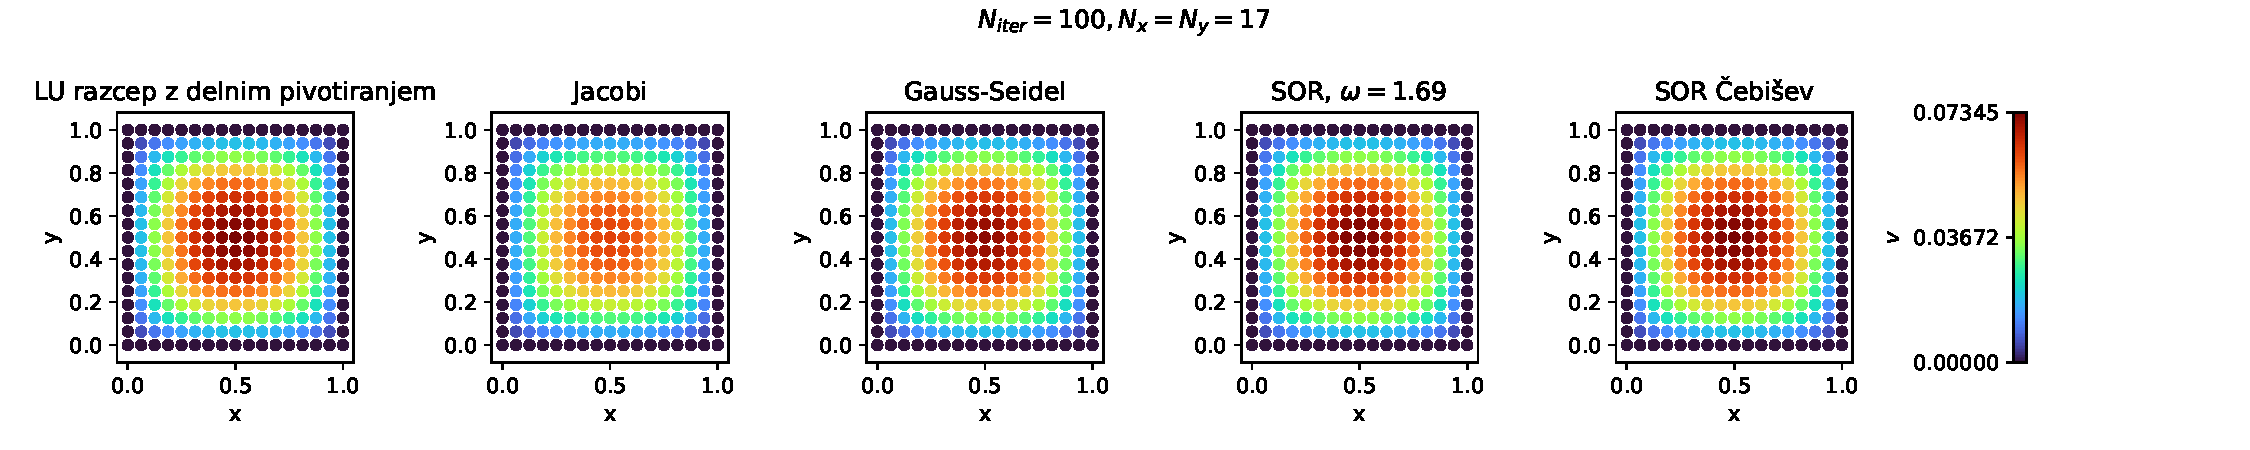
\includegraphics[width=\linewidth]{5.nal_slike/1.nal/kvadrat_Nx17.pdf}
    \end{subfigure}
    \begin{subfigure}{\textwidth}
        \centering
        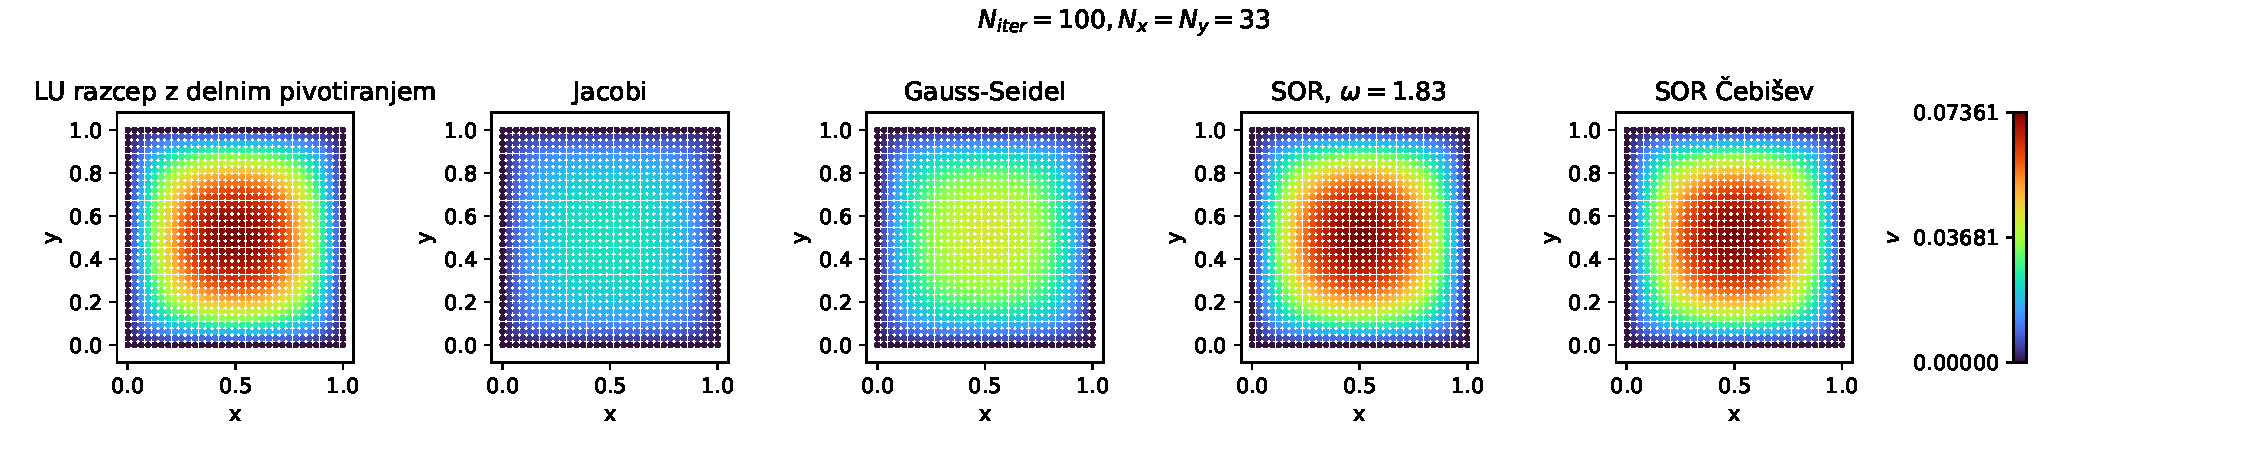
\includegraphics[width=\linewidth]{5.nal_slike/1.nal/kvadrat_Nx33.pdf}
    \end{subfigure}
    \caption{Hitrostni profil v kvadratni cevi pri 100 iteracijah}
\end{figure}

Pouiseuillov koeficient $C$ predstavlja posplošen izračun pretoka skozi cevi neokroglega prereza, glede na analitično rešitev hitrotnega profila okrogle cevi. 
\begin{equation}
    \dot V = C\,\frac{A^2\,dp}{8\,\pi\,\eta},
\end{equation}
kjer je $\dot V = \int_A \,v(x,y) \,dA$ volumski pretok, za izračun katerega sem uporabil Rombergovo metodo, $dp=1$ enotski tlačni gradient, $\eta=1$ enotka viskoznost in $A$ prečni presek cevi.

Za 100 iteracij vsake metode je prikazan rezultat za izračunan koeficient $C$, kjer je opazno, kako pri večjem številu točk rešitev ni pravilna za počasneje kopnvergiorajoče metode. Za Jacobi in Gauss-Seidlel bi moral povečati število iteracij. Iz SOR pa je koeficient dovolj stabilen.

\begin{figure}[ht]
    \centering
    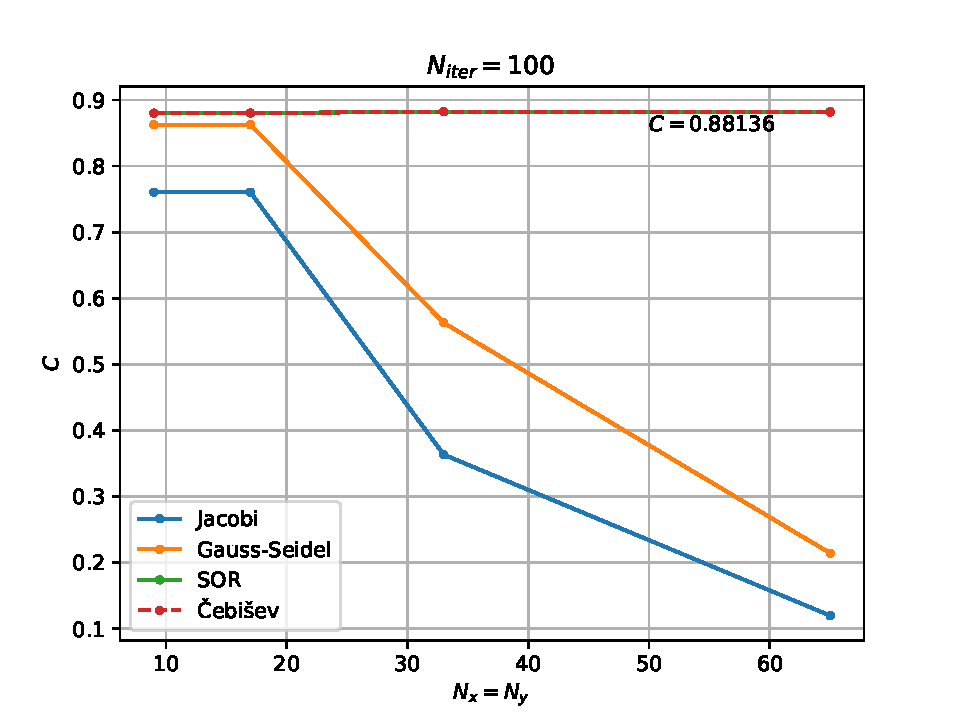
\includegraphics[width=0.5\linewidth]{5.nal_slike/1.nal/100iter_kvadrat_C.pdf}
    \caption{Pouiseuillov koeficient za kvadratno cev}
\end{figure}
  
\subsection{Poseben prerez}

Za cev drugačnega prereza, podano v navodilih naloge, sem izvedel toliko iteracij, da je bil residual med eksaktno in rešitvijo po iteraciji manjši od 1, tako sem dobil primerjive rešitve, kje je opazno, da je metoda SOR očitno hitrješa, vendar Čebišev pospešek ne prispeva bistveno. V tem primeru sem uporabljal oceno za $\omega$ po enačbi \ref{eq:omega}.

\begin{figure}[ht]
    \centering
    \begin{subfigure}{\textwidth}
        \centering
        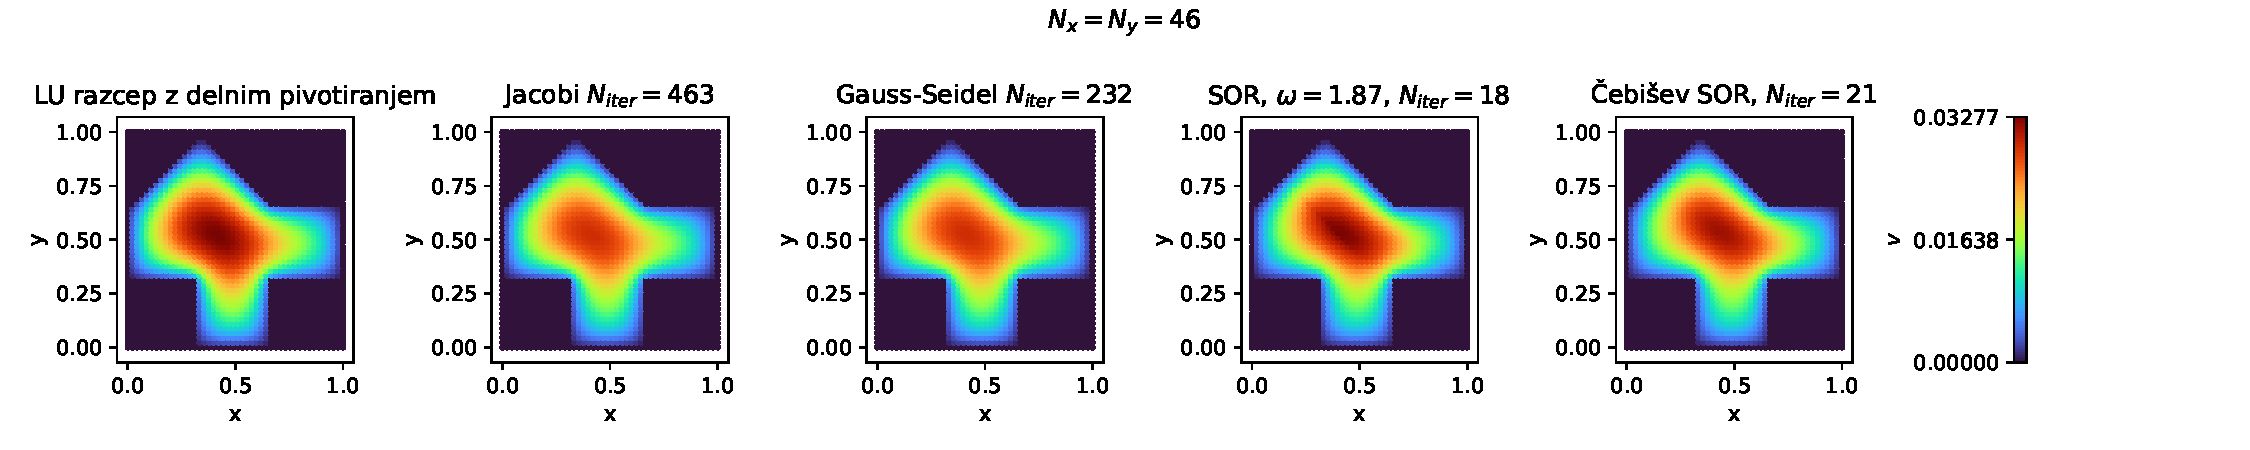
\includegraphics[width=\linewidth]{5.nal_slike/1.nal/cev_nal_Nx46.pdf}
    \end{subfigure}
    \begin{subfigure}{\textwidth}
        \centering
        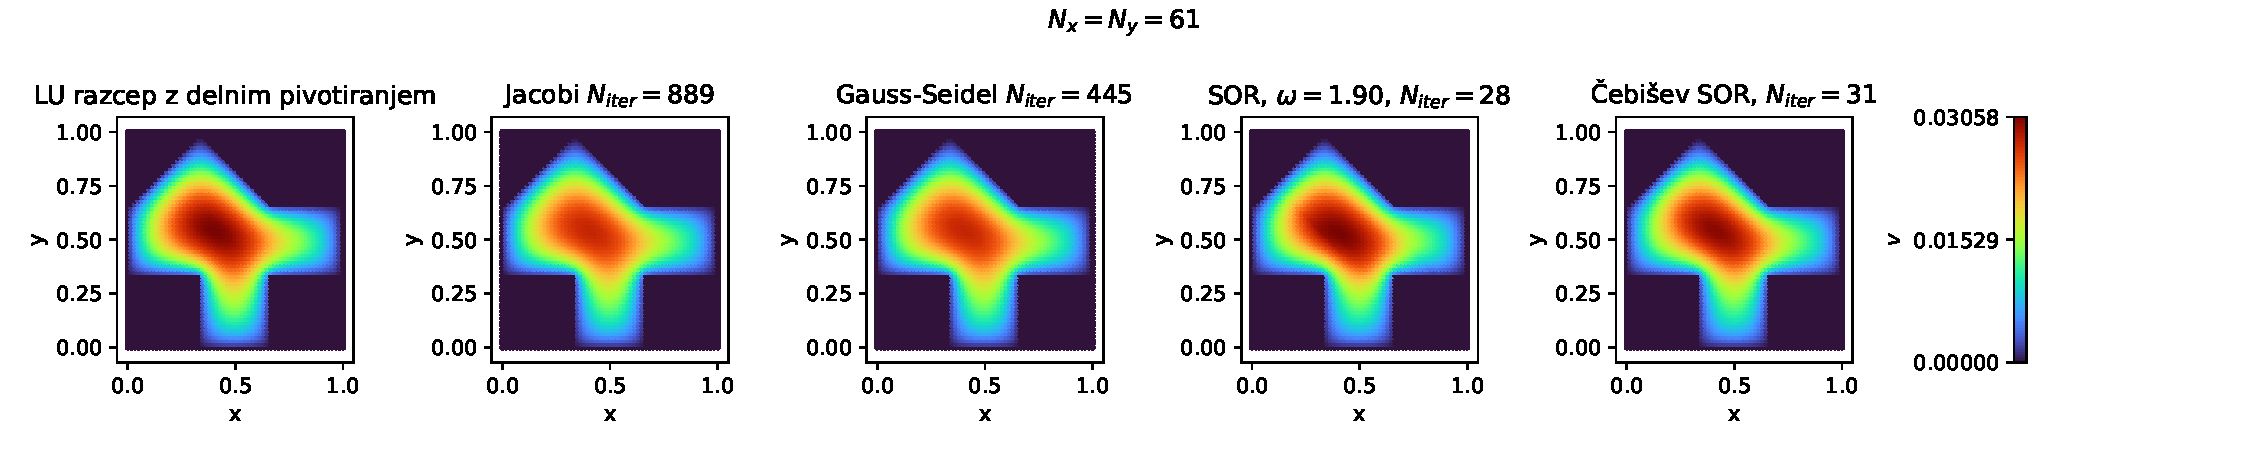
\includegraphics[width=\linewidth]{5.nal_slike/1.nal/cev_nal_Nx61.pdf}
    \end{subfigure}
    \caption{Hitrostni profil v cevi do residuala, manjšega od 1, glede na eksaktno rešitev}
\end{figure}

Boljšo oceno za $\omega$ nekvadratnih cevi dobimo po enačbi z utežjo $\alpha$
\begin{equation}
    \omega = \frac{2}{1+\alpha\,\frac{\pi}{N}},
\end{equation}
vendar je potrebno utež pravilno določiti glede na presek cevi.

Uporabil sem metodo za iskanje minimuma skalarne funkcije Brent v \\ \texttt{scipy.optimize.minimize\_scalar} in določil optimalen $\alpha$ za različna število točk. V splošnem se giblje okoli 1,5, rahlo padanje pa je mogoče posledica tega, da sem za izračun uporabil le 100 iteracij, kar zadošča za dovolj dobro rešitev eksaktni za mnjše število točk, pri večjem pa je odstopek večji, venda reda velikosti $10^{-2}$.

\begin{figure}[ht]
    \centering
    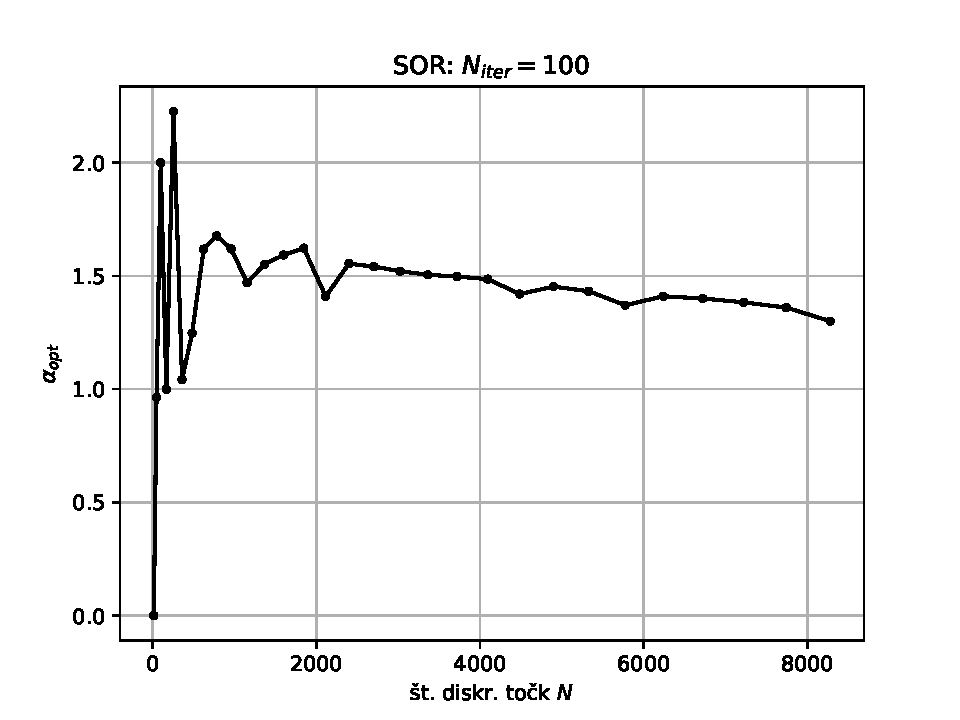
\includegraphics[width=0.75\linewidth]{5.nal_slike/1.nal/alpha_opt_Nx.pdf}
    \caption{Optimalen koeficient $\alpha$ pri oceni za $\omega$}
\end{figure}

Sedaj preprosto izračunam Pouiseuillov koeficient za vsako hitrostno polje na različno gosti mreži. Izračun prekinem, ko je sprememba po iteraciji za koeficient manjša od $10^{-10}$ in dobim sledeč graf, kjer je lepo vidna konvergenca. Špice sicer ne odstopajo pretirano, vendar mi vseeno ni jasno, od kod so prišle, morebiti bi moral še zmanjšati toleranco za koeficient.

\begin{figure}[ht]
    \centering
    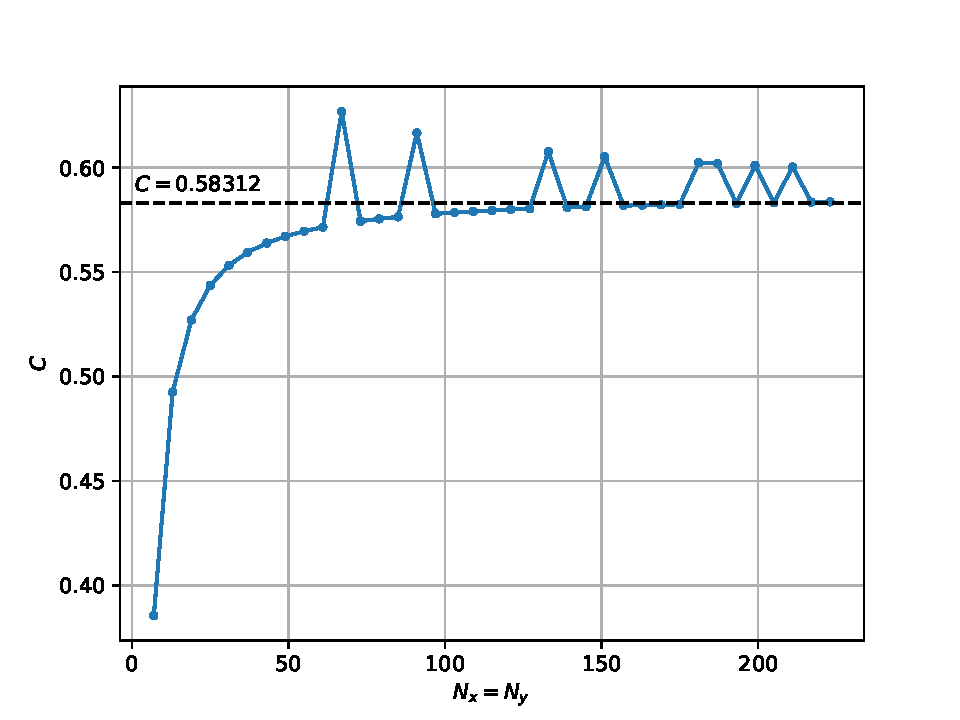
\includegraphics[width=0.75\linewidth]{5.nal_slike/1.nal/C_cev.pdf}
    \caption{Pouiseuillov koeficient za podano cev}
\end{figure}

%%%%%%%%%%%%%%%%%%%%%%%%%%%%%%%%%%%%%%%
\section{Prevod toplote po valju}

V drugi nalogi rešujem brezdimenzijsko obliko diferencialne enačbe prevoda toplote v stacionarnem stanju 
\begin{equation}
    \nabla^2 T = 0,
\end{equation}
ki se v cilindirčnem koordinatnem sistemu zapiše kot
\begin{equation}
    \frac{\partial^2 T}{\partial r^2} + \frac{1}{r}\,\frac{\partial{T}}{\partial r} + \frac{\partial^2T}{\partial{z^2}} =0,
\end{equation}
kjer zaradi osne simetrije obravnavam le prerez preko središča cilinda od plašča do sredine. Pri tem zapišem simetrijske robne pogoje na točkah na sredini $q(r=0)=0$, kjer je $q$ toplotni tok. Prav tako je Neumanov robni pogoj tudi na dnu cilindra $q(z=0)=2$ zaradi boljše vidljivosti.

Diricletovi RP so na zgornji ploskvi $T(z=1)=T_1$ in na plašču, kjer je na spodnji polovici $T(r=1, z<1/2)=T_1$ in na zgornji $T(r=1,z\leq1/2)=T_2$.

Na spodnji sliki sta prikazana različna primera takih robnih pogojev na plašču. Zanimivo je, da za enako točno rešitev potrebnih manj iteracij SOR, če je $T_2>T_1$. Število iteracij je tolikšno, da je residual med rešitevijo po SOR in eksaktno za ploščo manjši od ena. V tem primeru sem namreč opazil, da ob upoštevanju radialnega člena v diferencialni enačbi Gaussova eliminacija odpove, zato sem rešil sistem brez radialnega dela, kar torej predstavlja ploščo. Presenetljivo pa je bila ta rešitev zelo podobna onim z iterativnim reševanjem v cilindirnem koordinatnem sistemu. Opazno je tudi, koliko je SOR hitrejši od preostalih dveh metod. Parameter $\omega$ sem ocenil po enačbi \ref{eq:omega}.

\begin{figure}[H]
    \centering
    \begin{subfigure}{\textwidth}
        \centering
        \includegraphics[width=\linewidth]{5.nal_slike/primerjava_metod_Trp1_1_Trp2_0.pdf}
        \caption{Plašč zgoraj hladnejši, $T_1=1$, $T_2 = 0$}
    \end{subfigure}
    \begin{subfigure}{\textwidth}
        \centering
        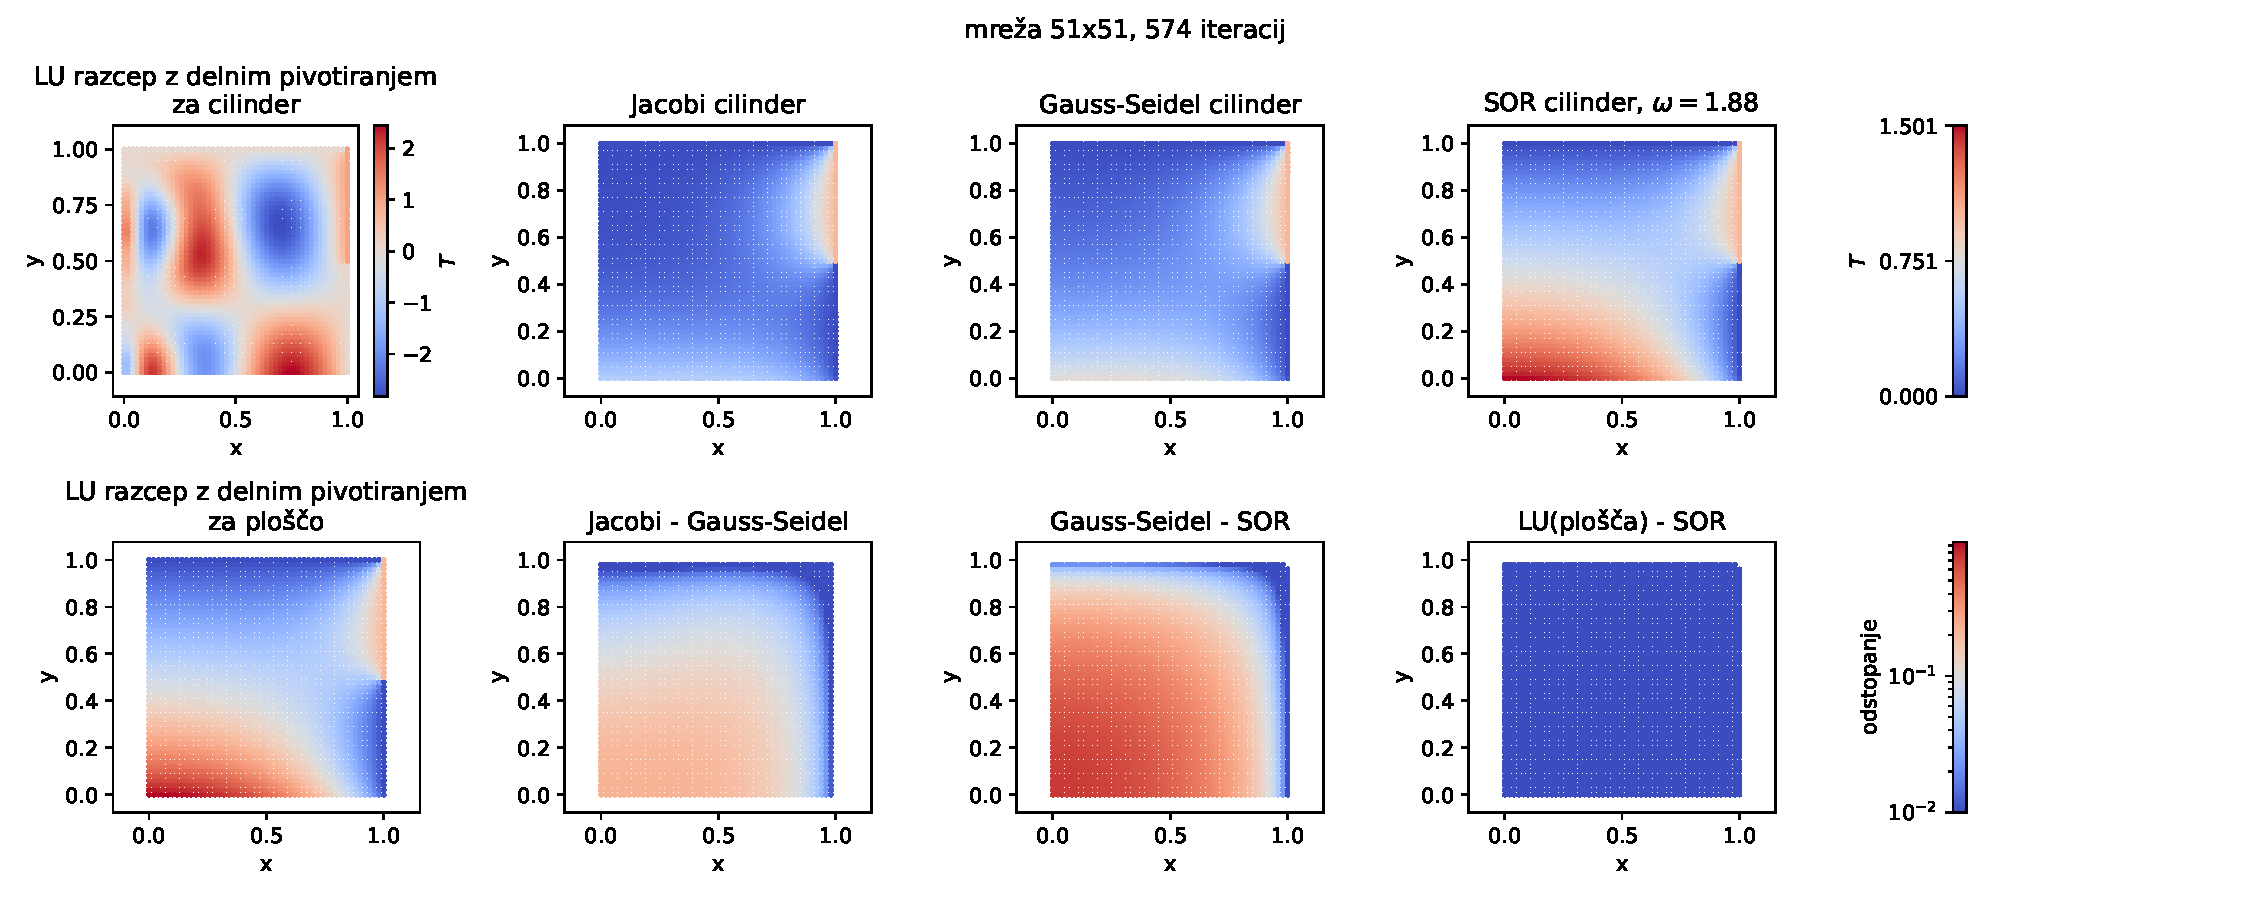
\includegraphics[width=\linewidth]{5.nal_slike/primerjava_metod_Trp1_0_Trp2_1.pdf}
        \caption{Plašč zgoraj toplejši, $T_1=0$, $T_2 = 1$}
    \end{subfigure}
    \caption{Robni pogoji po navodilih}
\end{figure}

Poigral sem se še z robnimi pogoji in predpostavil idealno toplotno izolirano cev namesto Dirichletovega $T_2$, torej $q=0$, prikazano na sliki \ref{fig:zgoraj_izol} in popolnoma izolirano desno stran na sliki \ref{fig:izol}, kar lahko v bistvu obravnavamo kot enodimenzijski prevod toplote. Ponovno Gaussovo eliminacijo zmoti radialni člen.

\begin{figure}[H]
    \centering
    \begin{subfigure}{\textwidth}
        \centering
        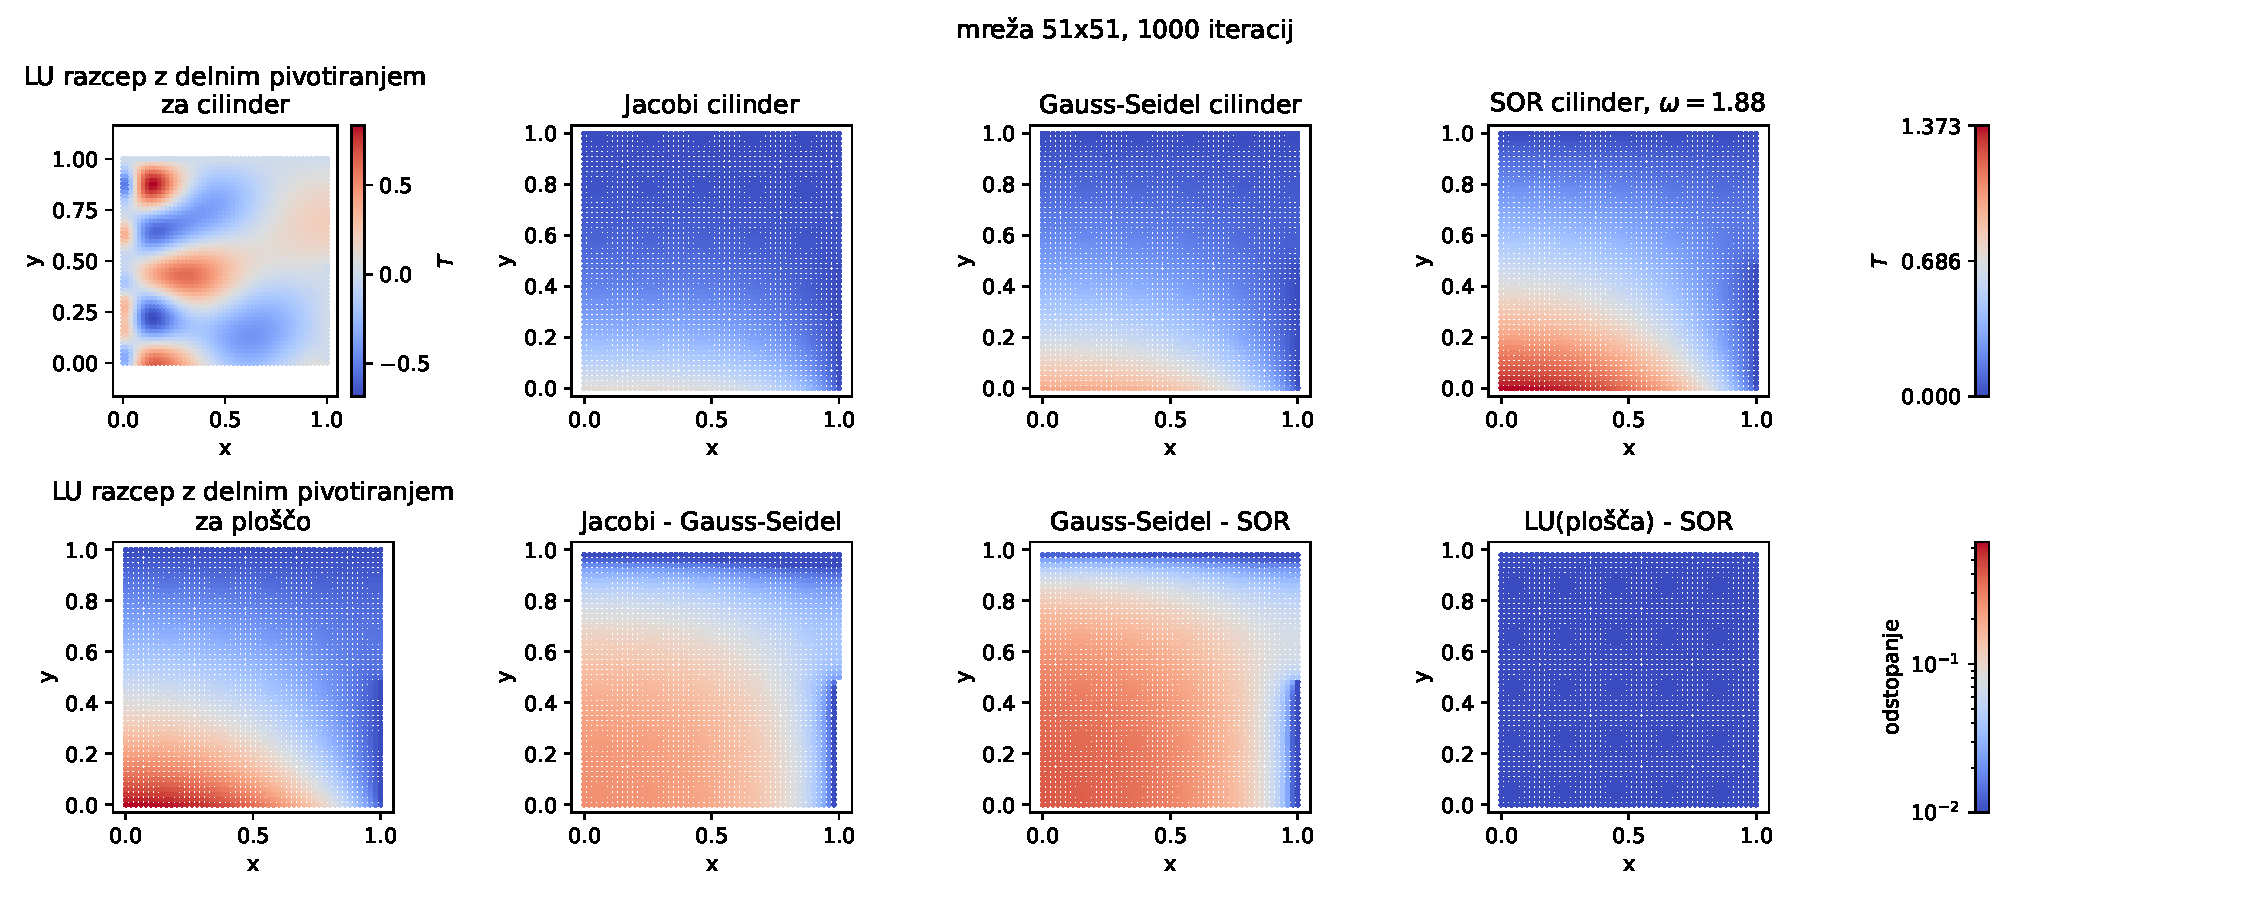
\includegraphics[width=\linewidth]{5.nal_slike/primerjava_metod_zdesno_goraj_izolirano_N50_1000iter.pdf}%drugje RP temp.
        \caption{desno zgoraj idealno izolirana cev}\label{fig:zgoraj_izol}
    \end{subfigure}
    \begin{subfigure}{\textwidth}
        \centering
        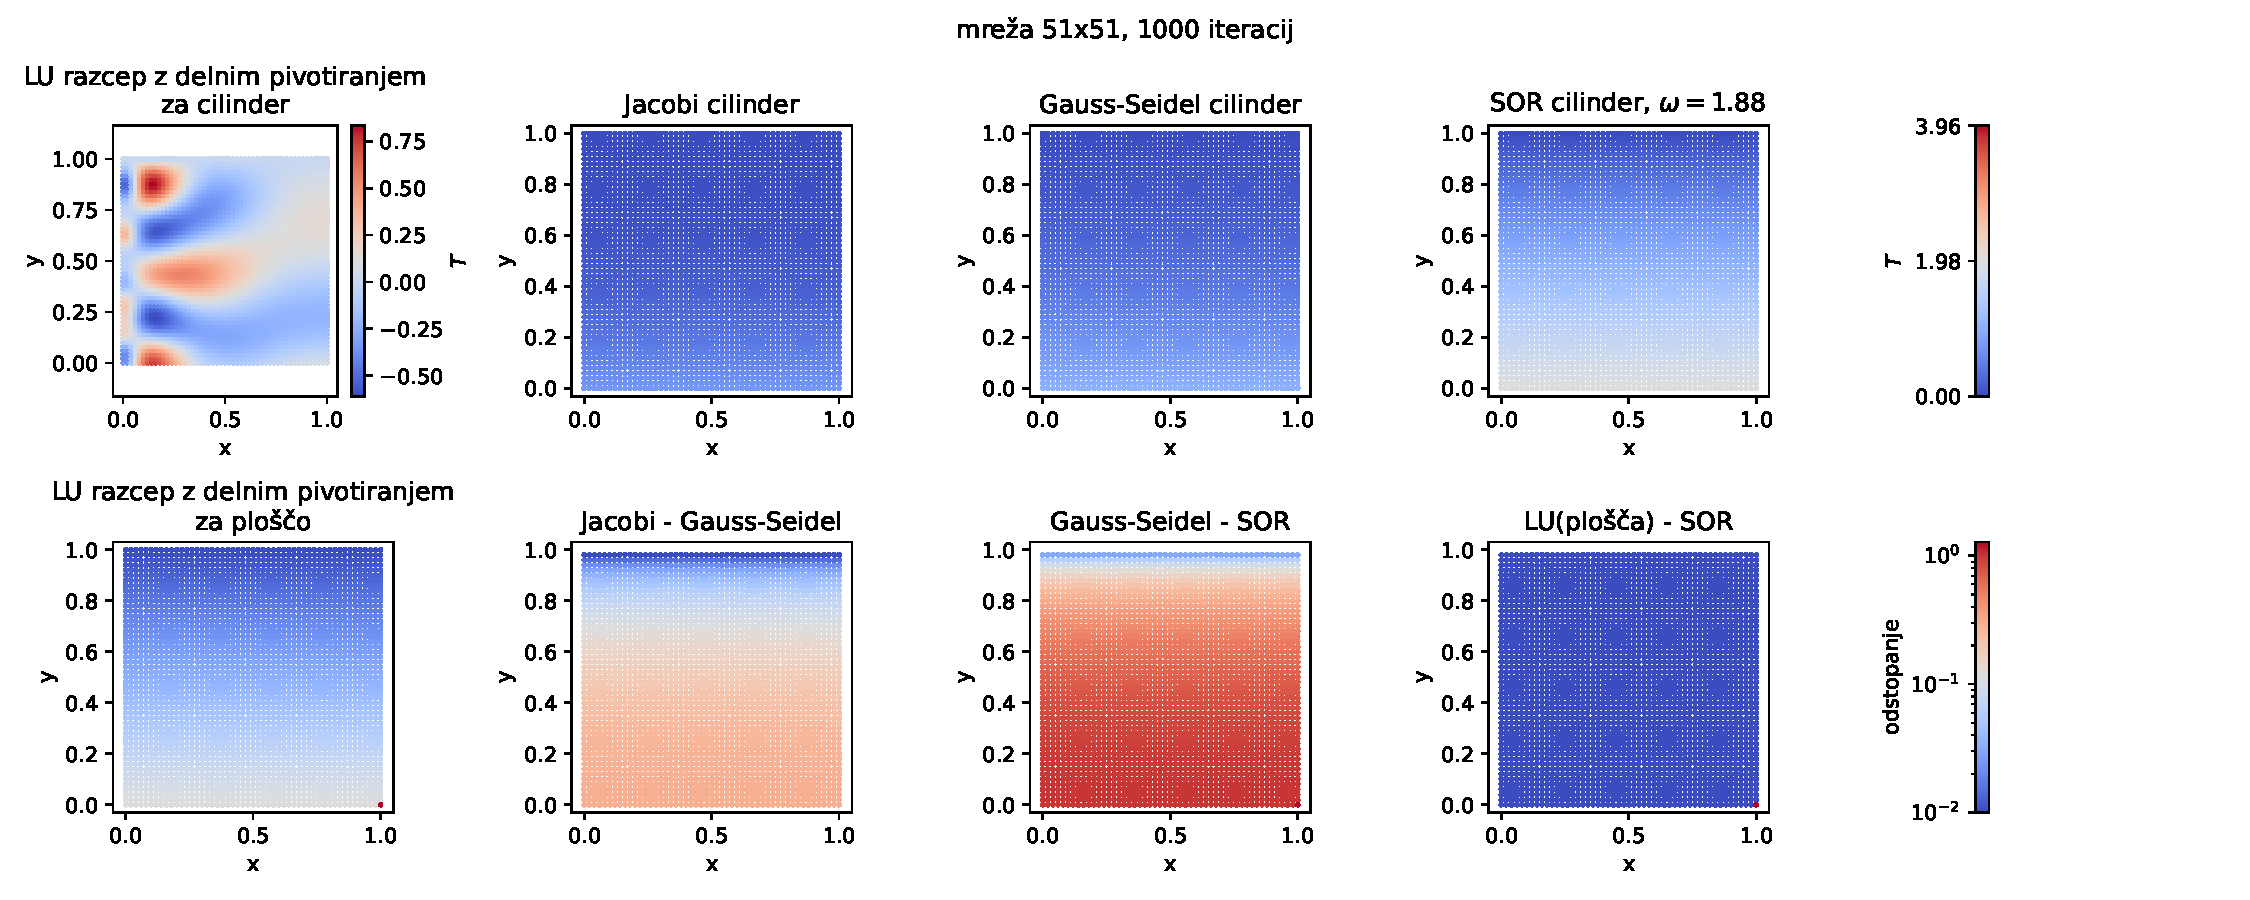
\includegraphics[width=\linewidth]{5.nal_slike/primerjava_metod_desno_izolirano_N50_1000iter.pdf}%desno vse izolirano! zgoraj RP temp.
        \caption{idealno izolirana cev po celem plašču}\label{fig:izol}
    \end{subfigure}
    \caption{Drugačni robni pooji}
\end{figure}

Za probleme prevoda toplote je uporabna tudi metoda končnih/kontrolnih volumnov (MKV), zato sem izračunal prevod toplote v 2D za ploščo, vendar prihaja do odstopanj med MKV in MKR predvsem v spodnjih dveh ogliščih. To je verjetno posledica, da se pri MKV Dirichletove robne pogoje aproksimira s toplotnim tokom preko meje kontrolnega volumna.Izračuni so izvedeni na mreži 51x51, kjer so v kontrolni volumni postavljeni s središčem v računski točki za MKR.

\begin{figure}[H]
    \centering
    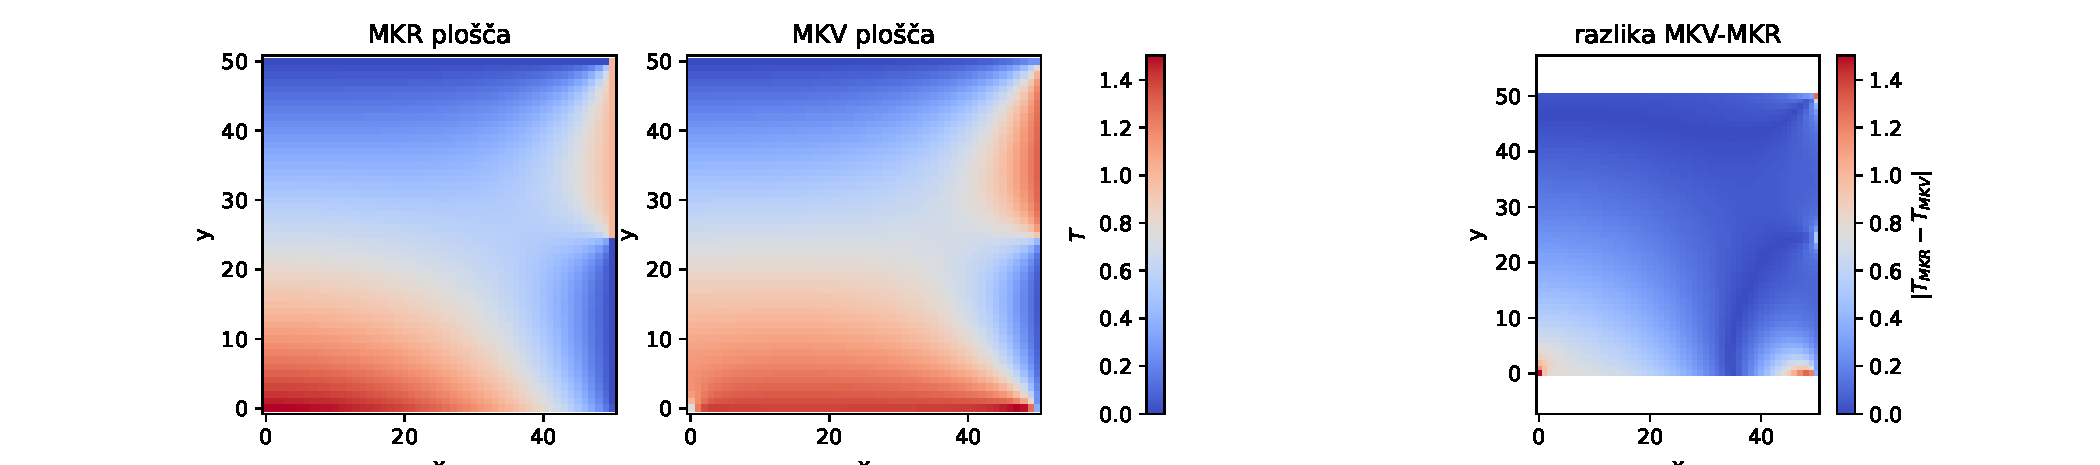
\includegraphics[width=\textwidth]{5.nal_slike/MKV.pdf}
    \caption{Primerjava med rešitvijo za ploščo po MKV in MKR}
\end{figure}

Tudi z bolj razširjeno metodo končnih elementov (MKE) je mogoče reševati diferencialno enačbo prevoda toplote. V tem primeru so robni pogoji tako primarne (temperatura), kot tudi sekundarne spremenljivke (toplotni tok) eksaktno izpolnejni, dočim so pri MKR le za primarno in MKV za sekundarno spremenljivko.

Izračuni so bili izvedeni s programom \textit{Ansys 2024 R1} in sicer za ploščo v 2D in z 90 000 končnimi elementi ter za cilinder v 3D in z 107 000 končnimi elementi. V tem primeru je najlepše vidna razlika med ploščo in cilindrom, ki je predvsem v spodnjem delu, kjer je robni pogoj za vstopajoč toplotni tok, vendar še vedno ne pojasnjuje čudnih rešitev, dobljenih z Gaussovo eleimenacijo.

\begin{figure}[ht]
    \centering
    \begin{subfigure}{0.45 \textwidth}
        \centering
        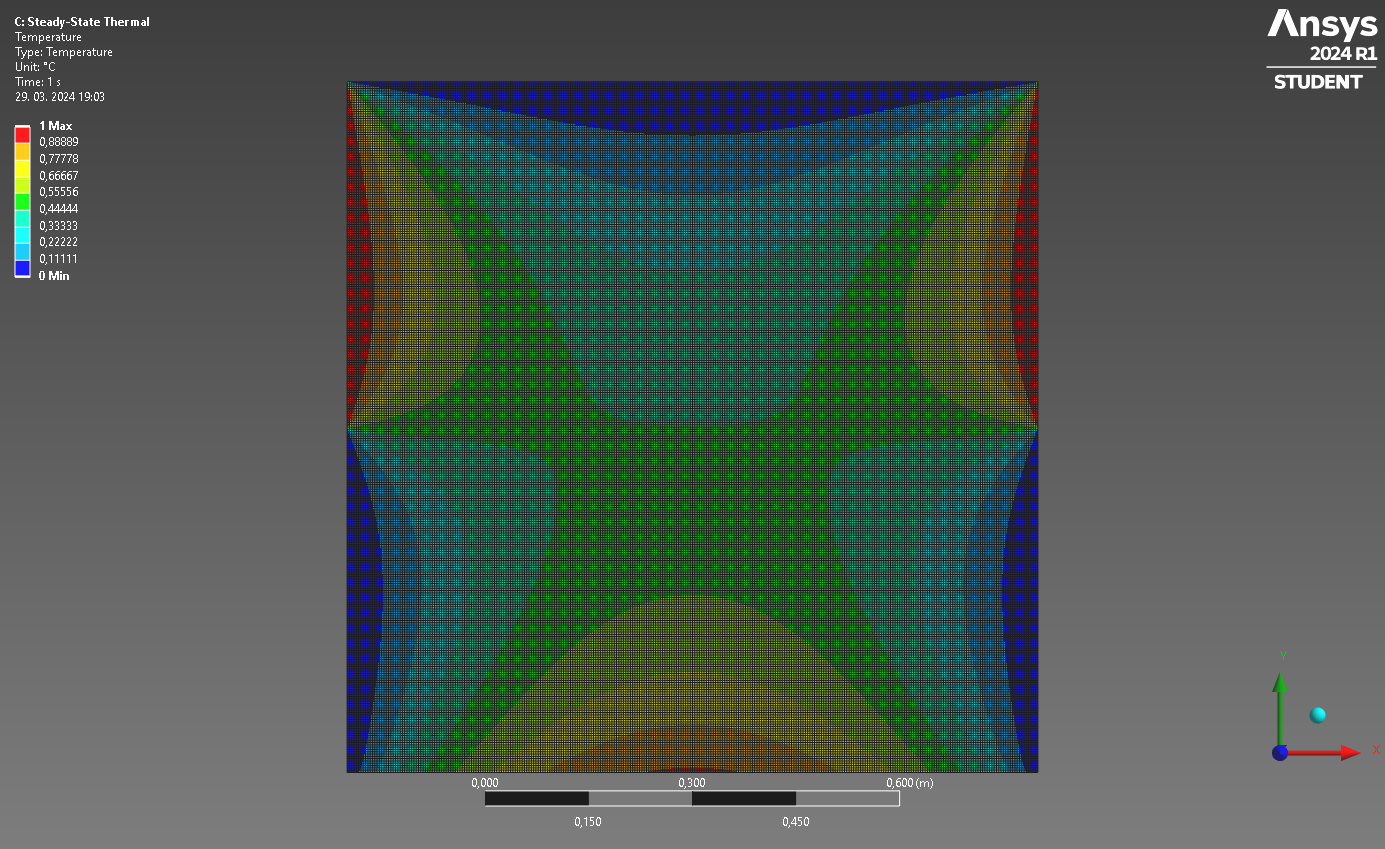
\includegraphics[width=\linewidth]{5.nal_slike/2D_90k_plosca.png}
        \caption{plošča}
    \end{subfigure}
    \begin{subfigure}{0.45\textwidth}
        \centering
        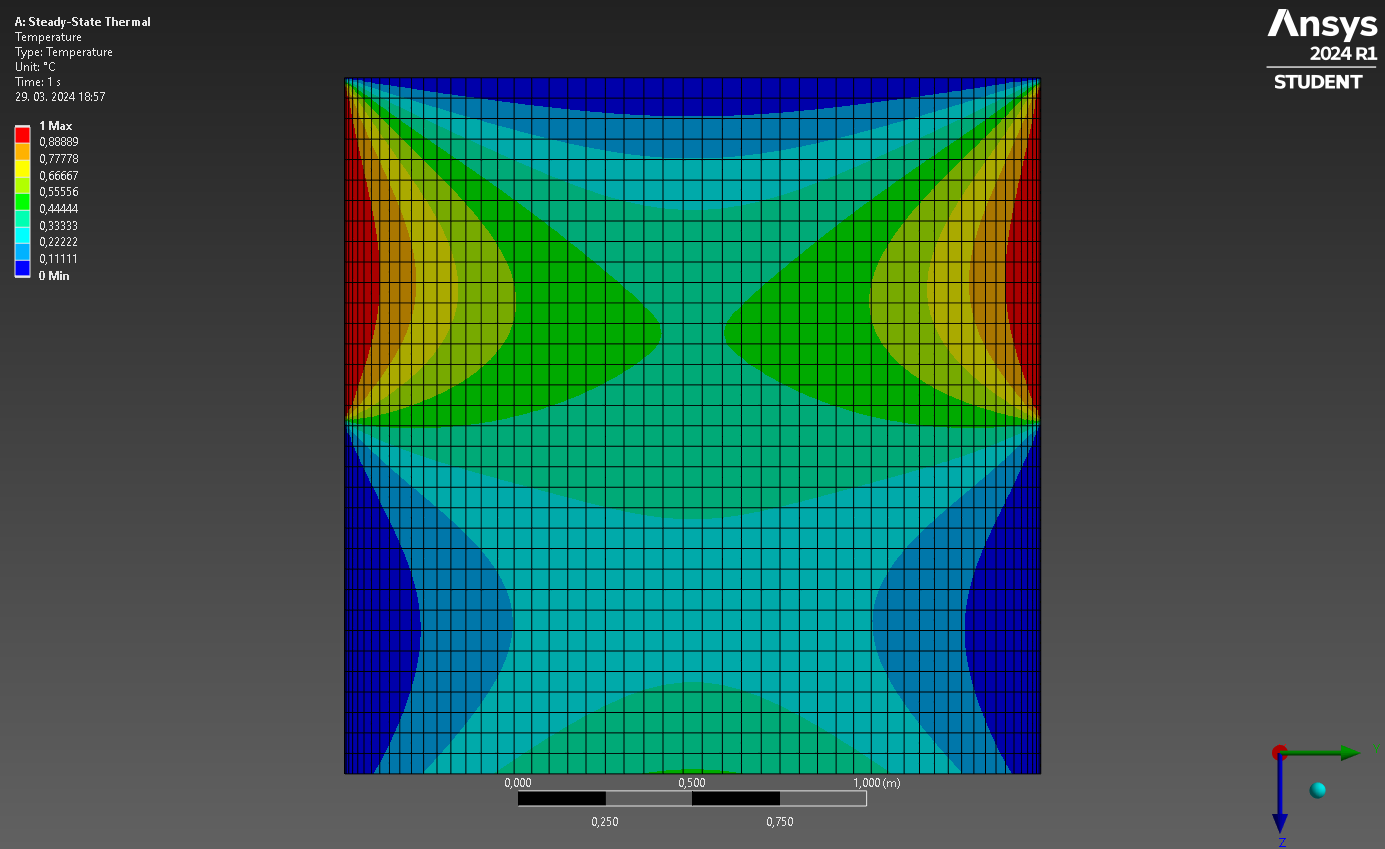
\includegraphics[width=\linewidth]{5.nal_slike/3D_107k.png}
        \caption{cilinder}
    \end{subfigure}
    \caption{Rešitev po MKE}
\end{figure}

\subsection{Optimalen $\omega$}

Na spodnji sliki je prikazano, koliko iteracij je potrebnih za doseganje enako točnega rezultata pri različnih parametrih nad-relaksacije $\omega$.

Na levi sliki sem rezultat po iteraciji primerjal z eksaktno rešitvijo $T_{ref}$ sistema enačb brez radialnega člena (plošča). Prikazanih je število iteracij $N$, potrebnih, da je residual $|T_{N}-T_{ref}| < 1$.

Na desni sliki pa sem prvo izvedel 10 iteracij vsake metode in nato izvedel toliko iteracij, da je bilo izboljšanje rešitve za 1.3 glede na izhodiščno $||\frac{T_{ref}-T_{N}}{T_{ref}}|| < 1$, kjer je $T_{ref}$ rešitev po prvih 10 iteracijah.

Nekako se mi zdi, da tak način merjenja ni bil najboljši, saj se je vedno kot najbolje izkazala $\omega=2$. Tudi prvi način vrne sumljivo visoko $\omega$. Vseeno sem zadovoljen s potekom krivulje drugje, saj le-ta vedno pada, pri $\omega=1$ pa je število iteracij enako onemu pri Gauss-Seidlovem algoritmu, katero sem uporabljal kot prediteracijo pri SOR. Prav tako je lepo opazna 2x pohitritev Gauss-Seidla glede na Jacobija in upočasnitev pri zgoščevanu mreže.

\begin{figure}[ht]
    \centering
    \begin{subfigure}{0.49\textwidth}
        \centering
        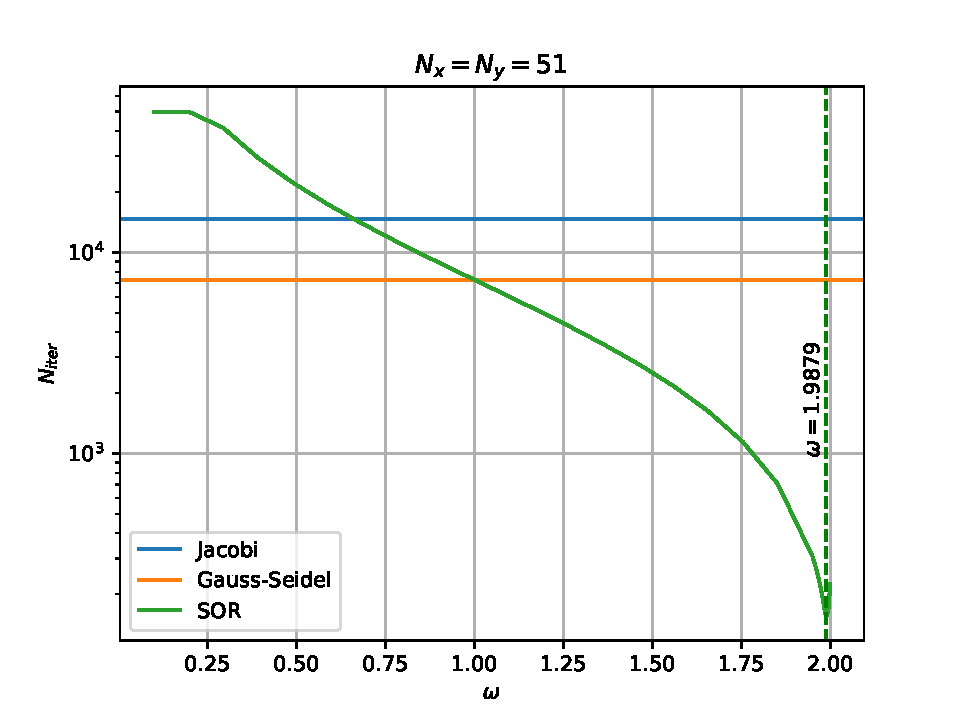
\includegraphics[width=\linewidth]{5.nal_slike/primerjava_LU.pdf}
        \caption{primerjava z eksaktno rešitvijo}
    \end{subfigure}
    \begin{subfigure}{0.49\textwidth}
        \centering
        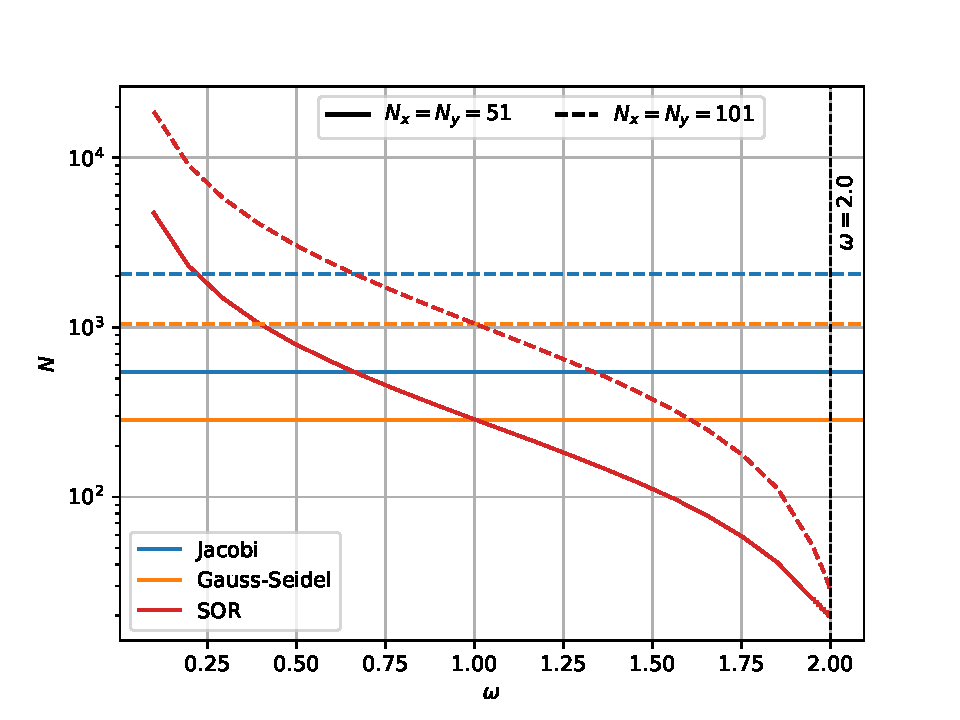
\includegraphics[width=\linewidth]{5.nal_slike/N_iter_dva_Nx.pdf}
        \caption{primerjava izboljšave začetnih 10 iteracij}
    \end{subfigure}
    \caption{Optimalen $\omega$}
\end{figure}

Sledi še prikaz konvergence, kjer sem prikazal absolutno izboljšavo iteracije glede na prejšnjo, kar sem računal iz residuala $||T_n-T_{n-1}||$. Opomba: prva iteracija je šteta kot iteracija nič.

Ta graf izgleda že lepše, ponovno je opazna 2x pohitritev Gauss-Seidla glede na Jacobija, bolj zanimivi pa so poteki metode SOR pri različnih $\omega$. Okoli 100. iteraciije je izboljšava ne glede na parameter $\omega$ precej podobna, prej razlike in nato pa razlike naraščajo. Prredvsem je izrazito hitrejše izboljševanje rešitve pri malo iteracijah (pod 100) za SOR metodo glede na ostali dve, vendar je tudi Gauss-Seidel nad Jacobijem.

Tokrat je opazno, da $\omega=2$ ni optimalna izbira, prav tako tudi 1.988, dobljen iz primerjave z eksaktno rešitvijo, ni najboljši, vendar vseeno boljši od naivne ocene po enačbi \ref{eq:omega}. Očitno je optimalna $\omega$ ravno nekje vmes, vendar mi je ni uspelo natančneje odkriti.

\begin{figure}[H]
    \centering
    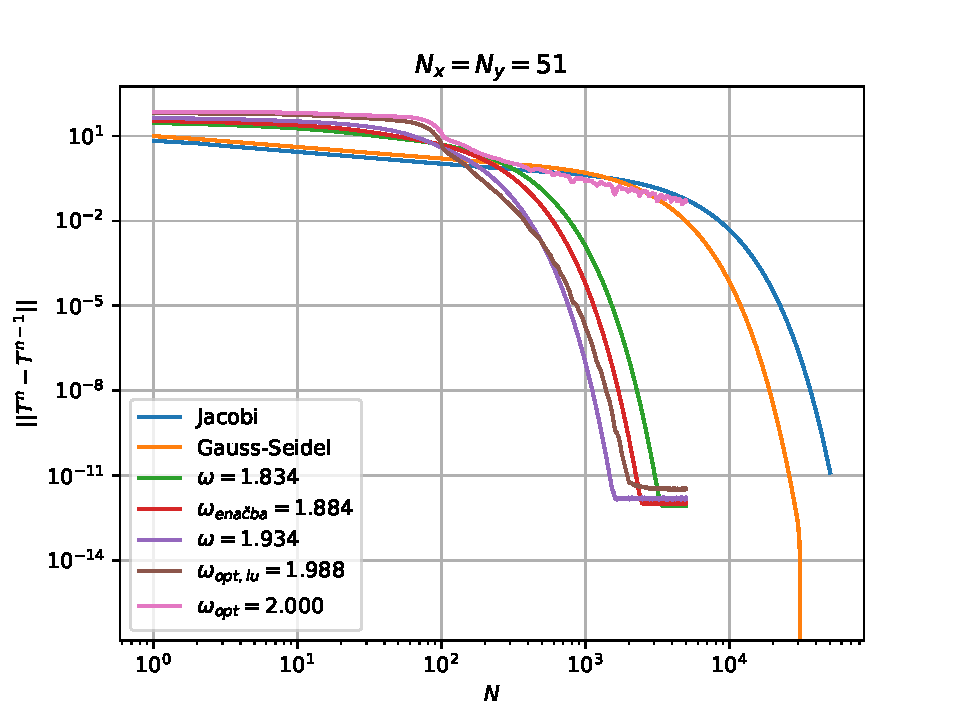
\includegraphics[width=0.7\linewidth]{5.nal_slike/izboljsava_iteracije.pdf}
    \caption{Doprinos iteracij k točnosti rešitve}
\end{figure}


\section{Zaključek}

Iterativne metode so sicer precej počasne in terjajo obravnavo robnih pogojev posebaj, saj lahko iteriramo le po središčnih točkah, kar je v primeru Neumanovih robnih pogojev bolj nepraktično. Za tako majhne probleme kot so bili v tej nalogi je direktno reševanje z Gaussovo eliminacijo hitrejše, če je le mogoče zaradi singularnosti v matriki. Iterativne metode so hitrejše od direktnega reševanja šele  primeru velikega števila neznank (pibl. nad $5\cdot 10^5$), vsekakor pa se splača uporabiti metodo SOR, saj smo za skoraj vsako $\omega>1$ hitrejši od Gauss-Seidlam, če le-ta ni preblizu $\omega=2$. Opazil sem tudi, da se z večanjem števila računskih točk (in posledično neznank) tudi parameter $\omega$ bliža proti vrednosti $\omega=2$.